\title{Lab Assignment 2 \\ \small{Datamining}}
\author{Chiel ten Brinke 3677133}
\documentclass[12pt]{article}
\usepackage{amssymb,amsmath,amsthm,enumerate,graphicx,float,lmodern,xparse}

\newtheorem{theorem}{Theorem}[section]
\newtheorem{lemma}[theorem]{Lemma}
\newtheorem{proposition}[theorem]{Proposition}
\newtheorem{corollary}[theorem]{Corollary}

\theoremstyle{definition}
\newtheorem{definition}[theorem]{Definition}
\newtheorem{axiom}[theorem]{Axiom}
\newtheorem{example}[theorem]{Example}
\newtheorem{remark}[theorem]{Remark}

%\newcommand{\set}[1]{\left\lbrace#1\right\rbrace}
%\newcommand{\set}[2]{\left\lbrace#1 \, \middle|\, #2 \right\rbrace}
\NewDocumentCommand\set{mg}{%
    \ensuremath{\left\lbrace #1 \IfNoValueTF{#2}{}{\, \middle|\, #2} \right\rbrace}%
}

\begin{document}
\maketitle

\section*{Notes}
\begin{itemize}
    \item There appeared to be a stupid error in the \texttt{gm.search} function which caused the algorithm to perform a first improvement local search rather than a best improvement local search as was required. I re-evaluated all computations and updated the report correspondingly.
The answers should be correct now.
    \item The tool I used to plot the 3d graph in question (h) appeared to be unavailable for some reason, so I redid this question entirely.
    \item The Bron-Kerbosch algorithm has not been taken from the site, but has been implemented manually.
\end{itemize}

\section*{Question A}
There are 10 variables, so there are $\frac{10 \cdot 9}{2} = 45$ undirected edges.
Since each combination of edges represents exactly one graphical model,
there are $2^{45} = 35184372088832$ possible graphical models.

\section*{Question B}
The table of counts has a cell for each combination of variable values.
This comes down to $9 \cdot 2 \cdot 2 \cdot 2 \cdot 3 \cdot 6 \cdot 4 \cdot 3 \cdot 5 \cdot 2 = 155520$ possible combinations.
This is confirmed by taking the length function of the table of counts in R.
The number of parameters of the saturated model equals the number of cells in the table of counts.

\section*{Question C}
\paragraph{Cliques}
$\set{1,3,10}$, $\set{1,8}$, $\set{1,9}$, $\set{2,8}$, $\set{2,9}$, $\set{2,10}$, $\set{3,6}$,
$\set{4,6}$, $\set{5,6}$, $\set{5,10}$, $\set{6,7}$, $\set{6,8}$, $\set{6, 9}$

\paragraph{BIC Score} 15841.66

\paragraph{Graph} See Figure~\ref{fig:c}

\begin{figure}[H]
    \centering
    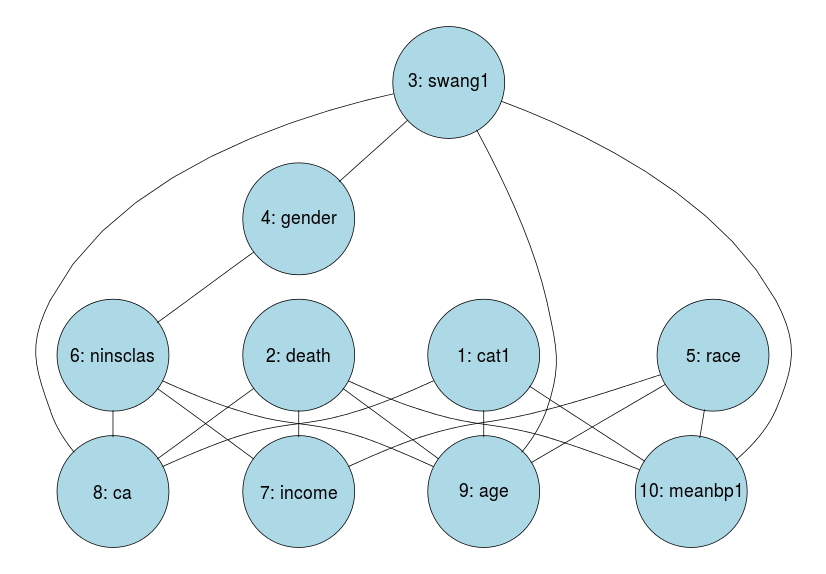
\includegraphics[width=0.8\linewidth]{c.png}
    \caption{Independence graph of backward forward search from empty graph using BIC.}
\label{fig:c}
\end{figure}

\section*{Question D}
\texttt{income} and \texttt{gender} are independent given \texttt{ninsclas}, because of the separator property.
To predict whether a patient will survive, we only need \texttt{ca}, \texttt{age} and \texttt{meanbp1}, because
\texttt{death} is independent of all other variables when these are given.

\section*{Question E}
\paragraph{Cliques}
$\set{1,3,10}$, $\set{1,8}$, $\set{2,7}$, $\set{2,8}$, $\set{2,9}$, $\set{2,10}$,
$\set{3,4}$, $\set{3,9}$, $\set{4,6}$, $\set{5,7}$, $\set{5,9}$, $\set{5,10}$,
$\set{6,7}$, $\set{6,8}$, $\set{6,9}$

\paragraph{BIC Score} 15850.53

\paragraph{Graph} See Figure~\ref{fig:e}

\begin{figure}[H]
    \centering
    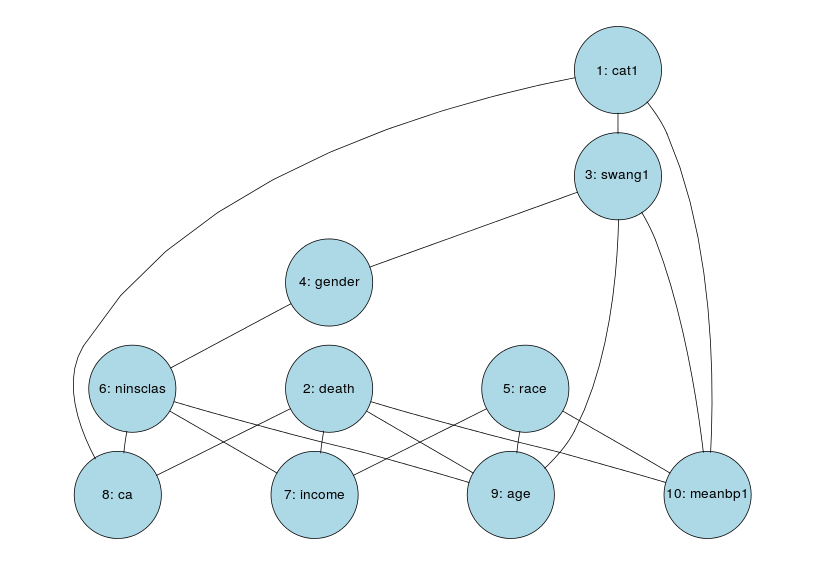
\includegraphics[width=0.8\linewidth]{e.png}
    \caption{Independence graph of backward forward search from complete graph using BIC.}
\label{fig:e}
\end{figure}

This model has a lower (thus better) BIC score than the model generated in c.
So this model is considered to be a better model.

\section*{Question F}
In both cases the algorithm gives the same result.

\paragraph{Cliques}
$\set{1,2,8}$, $\set{1,2,9}$, $\set{1,2,10}$, $\set{1,3,9}$, $\set{1,3,10}$, $\set{1,4,8}$,
$\set{1,4,10}$, $\set{3,6,9}$, $\set{4,5,6}$, $\set{4,5,10}$, $\set{4,8,6}$, $\set{7,2}$,
$\set{7,5,6}$, $\set{9,5,6}$

\paragraph{AIC Score} 14278.21

\paragraph{Graph} See Figure~\ref{fig:f}

\begin{figure}[H]
    \centering
    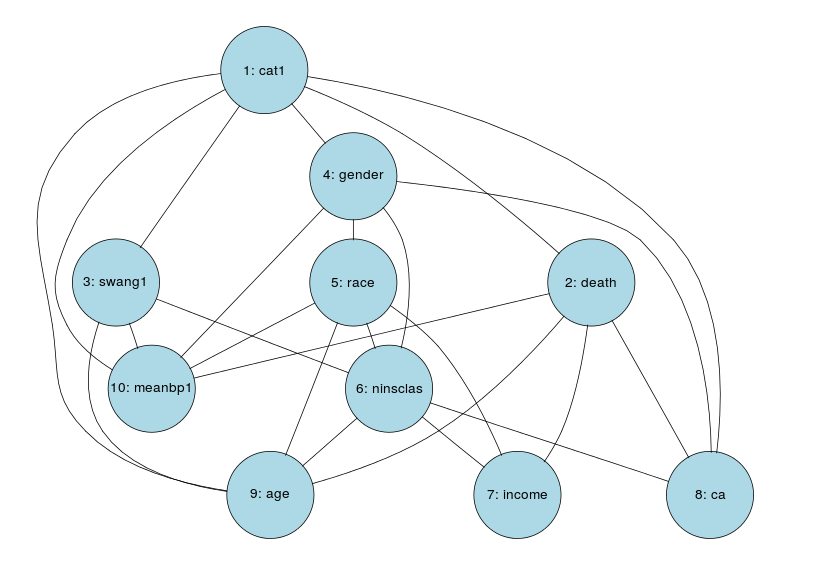
\includegraphics[width=0.8\linewidth]{f.png}
    \caption{Independence graph of backward forward search from empty graph or complete graph using AIC.}
\label{fig:f}
\end{figure}

%\subsection*{From complete graph}
%\paragraph{Cliques}
%$\set{1,2,8}$, $\set{1,2,10}$, $\set{1,4,3}$, $\set{1,4,8}$, $\set{1,6}$, $\set{1,10,3}$,
%$\set{7,2}$, $\set{7,3,4}$, $\set{7,5,6}$, $\set{8,2,9}$, $\set{8,4,9}$, $\set{9,3,4}$,
%$\set{9,5,6}$, $\set{10,5}$

%\paragraph{AIC Score} 14278.21

%\paragraph{Graph} See Figure~\ref{fig:f2}

%\begin{figure}[H]
    %\centering
    %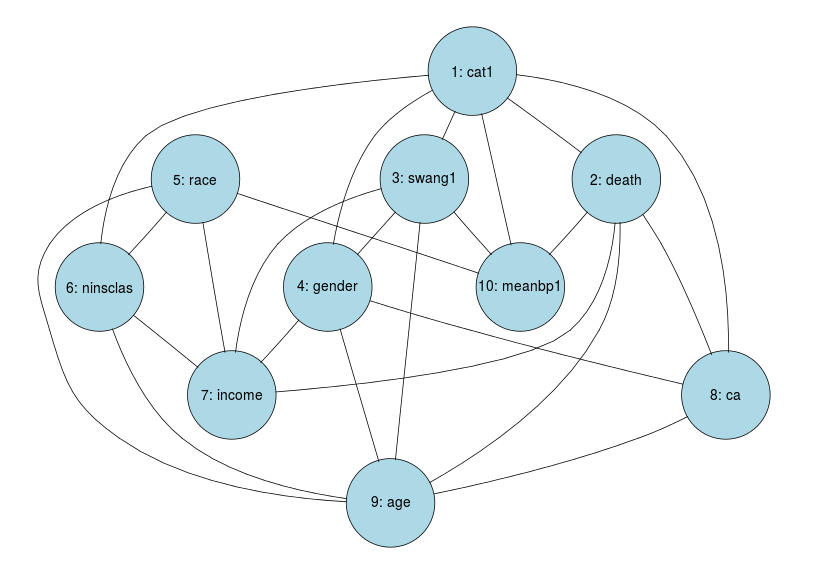
\includegraphics[width=0.8\linewidth]{f2.png}
    %\caption{Independence graph of backward forward search from complete graph using AIC.}
%\label{fig:f2}
%\end{figure}

%The two resulting models are almost the same, but there are some small differences.

\section*{Question G}
The models found with AIC are more complex than the models found with BIC.
This is because BIC penalizes complex models harder than AIC.

The models found with AIC are equal because it is more likely to find the
same model from the empty model if the penalty for complexity is low: it will
be less likely that the algorithm will stop because the model is too complex.

\section*{Question H}
The algorithm has been executed for several configurations of the parameters \texttt{nstart} and \texttt{prob} with respect to both AIC and BIC.
For each series of restarts the same seed has been used.
The findings have been plotted in level graphs which can be found in in Figure~\ref{fig:aic_plot} and Figure~\ref{fig:bic_plot} respectively.

\begin{figure}[H]
    \centering
    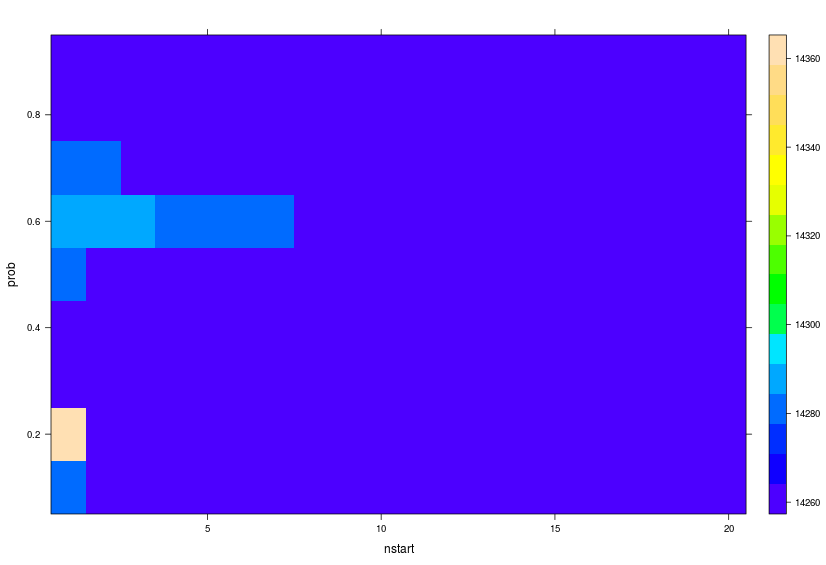
\includegraphics[width=0.8\linewidth]{aic_plot.png}
    \caption{AIC score as a function of \texttt{nstart} and \texttt{prob}.}
\label{fig:aic_plot}
\end{figure}

\begin{figure}[H]
    \centering
    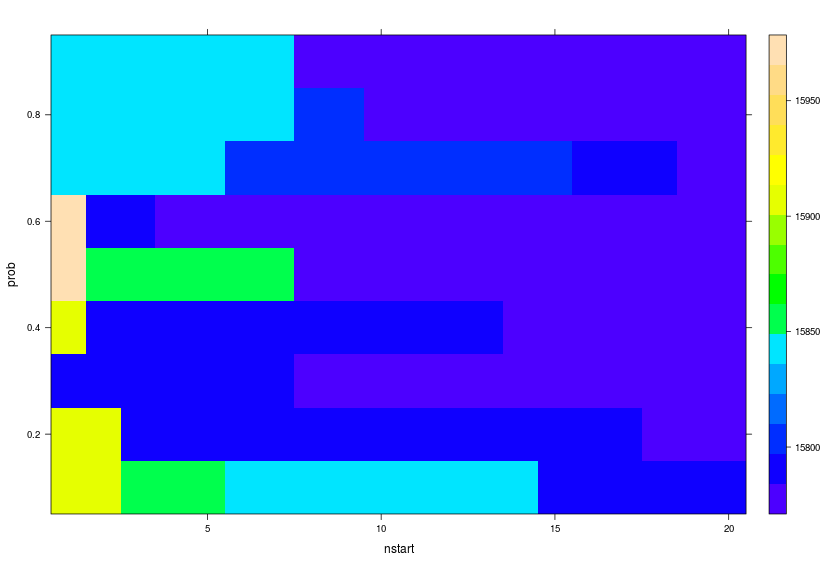
\includegraphics[width=0.8\linewidth]{bic_plot.png}
    \caption{BIC score as a function of \texttt{nstart} and \texttt{prob}.}
\label{fig:bic_plot}
\end{figure}

To get a reliable idea of the score distribution as function of \texttt{nstart} and \texttt{prob}, one should do muliple runs for each configuration of the parameters.
However, this takes much computational time and is outside the scope of this assignment.

One can immediately see that the score improves as \texttt{nstart} increases.
This is natural, as the result cannot get worse when more restarts are done.
Moreover, it is clear that the algorithm converges much faster with the AIC score than with the
BIC score.
The influence of \texttt{prob} on the score (both AIC and BIC) is less clear.
One observation that we can make from the graph is that choosing a low value for
\texttt{prob} doesn't seem to pay off well for the BIC score.

\subsection*{Model with best AIC score}
The model with the best AIC score that we've encountered is the following.

\paragraph{AIC Score} 14263.97

\paragraph{Graph} See Figure~\ref{fig:aic_best}

\begin{figure}[H]
    \centering
    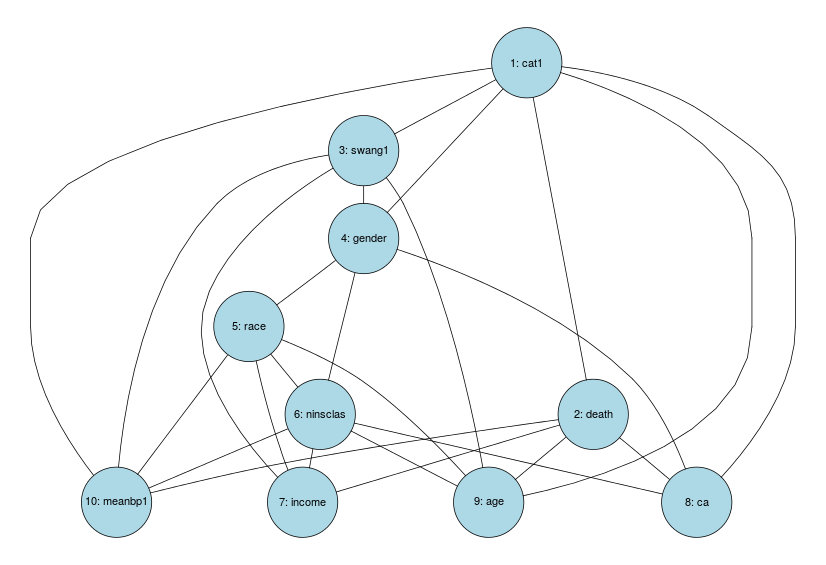
\includegraphics[width=0.8\linewidth]{aic_best.png}
    \caption{Independence graph of model with best AIC score.}
\label{fig:aic_best}
\end{figure}

\subsection*{Model with best BIC score}
The model with the best BIC score that we've encountered is the following.

\paragraph{BIC Score} 15783.74

\paragraph{Graph} See Figure~\ref{fig:bic_best}

\begin{figure}[H]
    \centering
    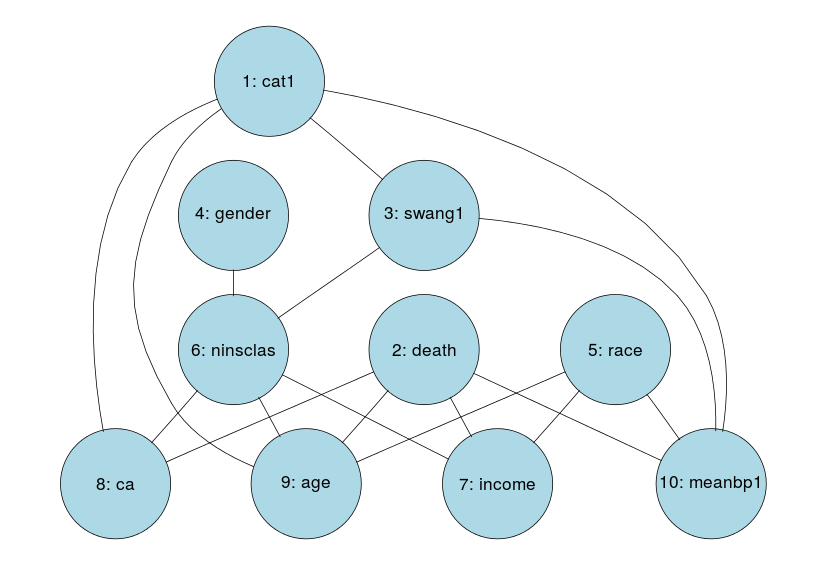
\includegraphics[width=0.8\linewidth]{bic_best.png}
    \caption{Independence graph of model with best BIC score.}
\label{fig:bic_best}
\end{figure}

\end{document}
